%%% Preamble
\documentclass[paper=a4, fontsize=11pt]{scrartcl}	% Article class of KOMA-script with 11pt font and a4 format
\usepackage[T1]{fontenc}
\usepackage{fourier}

\usepackage[english]{babel}															% English language/hyphenation
\usepackage[protrusion=true,expansion=true]{microtype}				% Better typography
\usepackage{amsmath,amsfonts}
\usepackage{amssymb}
\usepackage{amsthm}		
\usepackage{lscape}
\usepackage{hyperref}
\usepackage{algorithm}

\usepackage{algorithmicx}
\usepackage[noend]{algpseudocode}
\usepackage{mathtools}								% Math packages
\usepackage[pdftex]{graphicx}														% Enable pdflatex
\usepackage{url}
\linespread{1.1} % Line spacing
\usepackage[margin = 2.5cm]{geometry}


%%% Custom sectioning (sectsty package)
\usepackage{sectsty}												% Custom sectioning (see below)
\allsectionsfont{\centering \normalfont\scshape}	% Change font of al section commands


%%% Custom headers/footers (fancyhdr package)
\usepackage{fancyhdr}
\pagestyle{fancyplain}
\fancyhead{}														% No page header
\fancyfoot[L]{\small Team JS: Jonathan Irvin Gunawan and Khor Shi-Jie}		% You may remove/edit this line 
\fancyfoot[C]{}													% Empty
\fancyfoot[R]{\thepage}									% Pagenumbering
\renewcommand{\headrulewidth}{1pt}			% Remove header underlines
\renewcommand{\footrulewidth}{1pt}				% Remove footer underlines
\setlength{\headheight}{13.6pt}


%%% Equation and float numbering
\numberwithin{equation}{section}		% Equationnumbering: section.eq#
\numberwithin{figure}{section}			% Figurenumbering: section.fig#
\numberwithin{table}{section}				% Tablenumbering: section.tab#

\newtheorem{theorem}{Theorem}
\newtheorem{lemma}{Lemma}
\newtheorem{definition}{Definition}

%%% Maketitle metadata
\newcommand{\horrule}[1]{\rule{\linewidth}{#1}} 	% Horizontal rule

\title{
		%\vspace{-1in} 	
		\usefont{OT1}{bch}{b}{n}
		\normalfont \normalsize \textsc{CS5234 Combinatorial and Graph Algorithms} \\ [25pt]
		\horrule{0.5pt} \\[0.4cm]
		\huge Traveling Salesman Experiment \\
		\horrule{2pt} \\[0.5cm]
}
\author{
		\normalfont 								\normalsize
       Team JS: Jonathan Irvin Gunawan, Khor Shi-Jie\\[-3pt]		\normalsize
        \today
}
\date{}



%%% Begin document
\begin{document}
\maketitle

\section{Introduction}
The study of traveling salesman problem (TSP) is a natural generalization of the Hamiltonian cycle problem. We are interested to identify a cycle within a weighted graph such that the cycle includes all vertices in the graph and each vertex is only visited once in the cycle. In addition, we would to identify the Hamiltonian cycle with the minimum sum of edge weight. A close analogue to this problem is the Chinese postman problem which seeks to identify a tour of minimum weight that traverses each edge in the graph at least once. While the exact solution to the Chinese postman problem can be obtained in polynomial time, it is surprising that a subtle change in the requirement of the problem makes the Travelling Salesman Problem unsolvable in polynomial time. In particular, we note that

\begin{theorem}
TSP is NP-Hard.
\end{theorem}

\begin{proof}
We will reduce a directed Hamiltonian Cycle Problem into TSP. Given a directed graph $G$, we construct a weighted complete directed graph $G'$ which has the same vertices as $G$. In addition, we assign a weight of 1 to the edges in $G$ which were originally in $G'$, and a weight of $\infty$ otherwise. Suppose we found a solution to the TSP using graph $G'$ that has finite weight. Then, each of the edges must have weight 1 and hence must be present in the original graph $G$. As such, the solution to the TSP in $G'$ is also a solution to the Hamiltonian Cycle Problem in $G$. On the other hand, if the solution to TSP in $G'$ has infinite weight, then there is no Hamiltonian cycle which only consist of edge weight 1. Hence, there is no Hamiltonian cycle in $G$. As such, the directed Hamiltonian Cycle Problem reduces to TSP. Since the directed Hamiltonian Cycle problem is NP-Hard, TSP is also NP-Hard.
\end{proof}

There has been considerable research done in the past in determining the exact solution for TSP in a graph. A naive algorithm that checks all possible Hamiltonian cycle will incur $O(n!)$ time. It is possible to improve the runtime to $O(n^{2}2^n)$ using dynamic programming (i.e. Held-Karp algorithm), but even such algorithm will take significant time on graphs with small number of vertices\footnote{On a modern computer, it is possible to obtain the optimal solution using Held-Karp algorithm within 1 second for a graph with less than 18 nodes. \cite{steven} Any more vertices will incur a much higher runtime.}. Researchers have explored other approaches such as branch-and-bound algorithms and linear programming. Currently, the record for the highest number of vertices in a graph in which a TSP solution is found is approximately 85,900 nodes\footnote{Found by Applegate et al. using Concorde TSP Solver. \cite{appleman}}. Nevertheless, this is a small quantity compared to many real world instances of TSP.

Due to the impossibility of find a polynomial-time algorithm to solve TSP and the relevance of TSP to real life problems, there has been a lot of research that seeks to find an efficient approximation algorithm with a small approximation ratio. Within our course, we have explored several approximation algorithm to solve the TSP, including a 2-approximation algorithm\footnote{This algorithm only applies for a metric TSP. The same algorithm can be applied to obtain approximate solutions to M-R TSP and G-R TSP as these variants are equivalent.} based on constructing a minimum spanning tree (MST), and a 1.5-approximation algorithm that include the application of a minimum weight perfect matching algorithm. However, the effectiveness of these algorithms are only theoretical in nature. While the worst-case bounds for these algorithms are irrefutable, the optimality of these algorithm may differ from our expectations when we apply them to real world data (i.e. a 2-approximation algorithm may perform better on average than a 1.5-approximation algorithm). As such, this project aims to compare the suitability of various approximation algorithm when applied to graphs obtained from real world data or other random means. 

\section{Problem Formulation}

Generally, there are four variants of TSP that one can seek to solve. We can either have a graph in which the distance function is a metric, or a graph with a generic distance function. In addition, we can also choose to allow repeated vertices within our solution. The four variants are summarized in the table below:

\begin{table}[h]
\centering
\begin{tabular}{|c|c|c|}
\hline
\multicolumn{1}{|l|}{} & Repeats & No Repeats \\ \hline
Metric                 & M-R TSP & M-NR TSP   \\ \hline
General                & G-R TSP & G-NR TSP   \\ \hline
\end{tabular}
\end{table}

We have shown in class that M-R TSP, M-NR TSP and G-R TSP are equivalent. For our project, we are more interested in M-NR TSP as we are using data obtained from the real world. In addition, we will assume that the graph is non-directional, and the distance between any two vertices is well-defined. 

For this project, we will implement four different approximation algorithms and profile the performances on a set of random graphs and real world data. The four approximation algorithms are:
\begin{enumerate}
\item \textit{Nearest neighbour heuristics.} We start from a cycle with only one vertex in the cycle. Then, while there are vertices which are not included within our cycle, we choose a vertex which is closest our cycle. Then, we add the vertex to the cycle at a position whereby the increase in the length of the cycle is minimal. Once all the vertices are added to the cycle, we will obtain a $O(log n)$-approximate solution to the TSP (to be proven in the next section).  
\item \textit{Minimum spanning tree.} We will build a minimum spanning tree for the graph and conduct a DFS traversal on the graph. Within the DFS traversal, we will skip any vertices which has already been visited. This will produce a 2-approximate solution to the TSP (proven in class).
\item \textit{1.5-approximate algorithm.} After finding the minimum spanning tree of the graph, instead of conducting a DFS, we add edges to the graph until all vertices in the graph have even degree. Then, we can find an Eulerian tour for the graph. The edges to be added will be selecting using a minimum weight perfect matching algorithm such as a modified Edmond's Blossom algorithm.\cite{kolmogorov}
\item \textit{2-opt algorithm.} This algorithm makes use of the fact that a cycle without crossing is shorter than a cycle with crossing under the assumption of triangle inequality. We will refine any random cycle until there can be no more improvement to the weights. This algorithm is an $O(\sqrt{n})$-approximate algorithm on average case for a metric space. \cite{christian} In a normed vector space (which applies for the Euclidean metric), the algorithm is an $O(\log n)$-approximate algorithm. 
\end{enumerate}

We are interested in the optimality of the solution produced by the above four algorithms, as well as the runtime in producing the solutions. In particular, we want to know how well these algorithms will perform on random graphs and real world data. 

In our project, we will first implement methods to generate random graphs and prepare 5 such graphs for experimentation. Then, we will parse real world data from (to be confirmed) and (to be confirmed) and store them in a weighted graph. We will apply each approximation algorithm on our generated graphs and obtain the weight of TSP solution produced by each algorithm. Each algorithm will be executed thrice and the average runtime taken for the algorithms will be calculated. Upon collecting these data, we will compare the results and conclude on the effectiveness of each approximation algorithm.

\section{Algorithms and Theory}

In this section, we will describe the implementation of the four approximation algorithms proposed in the previous section. We will assume that the graph is stored as an adjacency list. 

\subsection{Nearest Neighbour Heuristic}

We will implement the version of nearest neighbour heuristics described in the pseudocode below:
\begin{algorithm}
\caption{Nearest Neighbour Heursitics}\label{neighbour}
\begin{algorithmic}[1]
\Procedure{Nearest-Neighbour-Heuristics}{$G = (V,E)$}\Comment{Returns the TSP approximation}
   \State Set $visited[v]\gets$ false, for all $v\in V$
   \State $TSP\gets\emptyset$
   \State $u_{0}\gets 1$ \Comment{Choose vertex 1 as the starting point}
   \State $u\gets u_{0}$
   \State $visited[u]\gets$ true
   \While{there are unvisited vertices}
      \State $v\gets$ unvisited vertex that is closest to $u$
      \State $TSP\gets TSP\cup(u,v)$
      \State $visited[v]\gets$ true
      \State $u\gets v$
   \EndWhile\label{nearestneighbourwhile}
   \State \textbf{return} $TSP\cup(u,u_{0})$
\EndProcedure
\end{algorithmic}
\end{algorithm}

For any walk $P$, define $cost(P)$ to be the total weight of edges included in walk $P$. We also define $d(u,v)$ to be the weight of the edge between $u$ and $v$ (which exists based on our assumption that our graph is complete). In addition, let $NNH$ be the tour returned by the algorithm given above. We will prove that:

\begin{theorem}
Algorithm \ref{neighbour} is an $O(\log n)$-approximation algorithm.
\end{theorem}

\begin{proof}
The proof is adapted from \cite{ravi}. For every vertex $u\in V$, let $l_{u}$ be the length of the edge leaving vertex $u$ to vertex $v$, which is the nearest unvisited vertex from $u$ from the tour generated by the nearest neighbour heuristic.
\item
Let $(x_1, x_2, \cdots, x_n)$ be a permutation of $\{i\mid 1\leq i \leq n\}$ such that $l_{x_i} \geq l_{x_{i+1}}$ for any $i$ satisfying $1\leq i\le n$. We first prove the following lemmas.
\begin{lemma}
For any pair of vertices $(u,v)$, $d(u,v)\geq \min(l_{u},l_{v})$
\end{lemma}
\begin{proof} Consider the following two cases:
\item
Case 1: If vertex $u$ was visited in $NNH$ before vertex $v$, then $v$ was a candidate for the closest unvisited vertex from $u$. Therefore, edge $(u,v)$ is no shorter than the edge leaving vertex $u$ in $NNH$. Since the edge that is chosen has weight $l_{u}$ due to the greedy property of the algorithm, we conclude that $d(u,v)\geq l_{u}\geq \min(l_{u},l_{v})$.
\item
Case 2: If vertex $u$ was visited in $NNH$ after vertex $v$, then $u$ was a candidate for the closest unvisited vertex from $v$. Therefore, edge $(u,v)$ is no shorter than the edge leaving vertex $v$ in $NNH$. Since the edge that is chosen has weight $l_{v}$ due to the greedy property of the algorithm, we conclude that $d(u,v)\geq l_{v}\geq \min(l_{u},l_{v})$.
\item Either case 1 or case 2 must be true. Therefore, $d(u,v)\geq \min(l_{u},l_{v})$
\end{proof}
\begin{lemma}

For any vertex $u$, $2l_{u}\leq OPT$
\end{lemma}
\begin{proof}
Consider breaking the optimal tour into two disjoint paths P and Q, where P starts from $u$ and ends at $v$, and Q starts from $v$ and ends at $u$. Note that, 
\[OPT = cost(P) + cost(Q)\]
Due to the triangle inequality, we note that $d(u,v)\leq cost(P)$ and $d(u,v)\leq cost(Q)$. Therefore, 
\[2d(u,v)\leq OPT\]
Hence, 
\[2l_{u}\leq OPT\]
\end{proof}
\begin{lemma}
For any $k$ satisfying $1\leq k\leq n$, $OPT\geq 2\sum\limits_{i=k+1}^{\min(2k,n)}l_{x_i}$
\end{lemma}
\begin{proof}
Let $H$ be the subgraph defined on the set of vertices $\{x_i\mid 1\leq i \leq \min(2k,n)\}$. Let $T$ be the tour in $H$ which visits the vertices in the same order as the optimal tour. By triangle inequality, every edge $(u,v)$ in $T$ have a length of less than or equal to the length of any path from $u$ to $v$ in the original graph. Therefore, 
\begin{align*}
OPT&\geq COST(T)\quad\text{ since $T$ is a part of $OPT$}\\
&\geq \sum\limits_{i=1}^{\min(2k,n)}\min(l_{x_i}, l_{x_{i+1}}) \quad\text{from Lemma 1. We assume that $x_{\min(2k, n)+1} = x_1$.}
\end{align*}
Note that each $l_{x_i}$ can appear at most twice in the summation above, since a vertex can only be the endpoint of at most 2 edges. We can attain the lower bound of the inequality by choosing the nodes with the smallest value for $l_{x_i}$. Using the fact that $l_{x_i} \ge l_{x_{i+1}}$ and since each node can only be chosen twice, we have
\[OPT\geq \sum\limits_{i=1}^{\min(2k,n)}\min(l_{x_i}, l_{x_{i+1}})\geq 2\sum\limits_{i=k+1}^{\min(2k,n)}l_{x_i}\]
\end{proof}
By Lemma 3
\begin{align*}
OPT &\geq 2\sum\limits_{i=k+1}^{\min(2k,n)}l_{x_i}\\
\sum\limits_{k=0}^{\lceil{\log n}\rceil-1}{OPT}&\geq \sum\limits_{k=0}^{\lceil{\log n}\rceil-1}\left(2\sum\limits_{i=2^{k}+1}^{\min(2^{k+1},n)}l_{x_i}\right)\\
&\geq 2\sum\limits_{k=0}^{\lceil{\log n}\rceil-1}\left(\sum\limits_{i=2^{k}+1}^{\min(2^{k+1},n)}l_{x_i}\right)\\
(\lceil\log n\rceil)OPT &\geq 2\sum\limits_{i=2}^{n}l_{x_i}
\end{align*}
By Lemma 2
\[OPT\geq 2l_{x_{1}}\]
Therefore,
\[(\lceil\log n\rceil+1)OPT\geq 2\sum\limits_{i=1}^{n}l_{x_i}\]
Therefore,
\[\frac{1}{2}(\lceil\log n\rceil+1)OPT\geq\sum\limits_{i=1}^{n}l_{x_i}\]
\[\frac{1}{2}(\lceil\log n\rceil+1)OPT\geq COST(NNH)\]
Therefore, $NNH$ is $O(\log n)$-approximation algorithm
\end{proof}

\subsection{Minimum Spanning Tree}
The construction of a 2-approximate tour using minimum spanning tree is exactly the same as the one introduced in lecture. As such, we will not restate the algorithm in this report. For this project, we will implement Kruskal's algorithm which generates a minimum spanning tree in $O(m \log n)$ time. This is sufficiently fast for a graph of no more than $10,000$ vertices.

To generate the MST for a graph of size more than $10,000$ vertices, we need to make use of the fact that the graphs which we will be analysing are complete, metric graphs. In this case, it can be proven that the minimum spanning tree of the graph is the minimum spanning tree of every Delaunay triangulation of the graph.\cite{sedgewick} It is possible to generate the Delaunay triangulation of a graph in $O(n \log n)$ time. Since the triangulated graph is planar, it only has $O(n)$ edges. Running Kruskal's algorithm on the new graph will yield a runtime of $O(n \log n)$. The total runtime for the algorithm will be $O(n \log n)$, which can be used to process graphs with size up to 1,000,000 vertices comfortably.
\subsection{2-opt Algorithm} The 2-opt algorithm is an approximation algorithm that seeks to improve on the weight of a given tour. Suppose we have already found a tour $x_1x_2\cdots x_nx_1$ for the given graph. For every pair of numbers $i, j$ that satisfy $1 < i+1 < j \le n$, we can construct a new tour $x_1x_2 \cdots x_ix_jx_{j-1} \cdots x_{i+1}x_{j+1}x_{j+2} \cdots x_n$. This new cycle is formed by deleting the edges $(x_i, x_{i+1})$ and $(x_j, x_{j+1})$, and adding the edges $(x_i, x_j)$ and $(x_{i+1}, x_{j+1})$. As such, there will be an improvement on the length of the tour if 
\[d(x_i, x_j) + d(x_{i+1}, x_{j+1})< d(x_i, x_{i+1})+d(x_j, x_{j+1}).\]

The 2-opt algorithm is described in the following pseudocode:

\begin{algorithm}
\caption{2-opt Algorithm}\label{2-opt}
\begin{algorithmic}[1]
\Procedure{2-Opt-Algorithm}{$G = (V,E)$}\Comment{Returns the TSP approximation}
   \State $TSP \gets $ Random Tour in $G$
   \While{$TSP$ was improved}
	\State  $i \gets 1$
	\State  $j \gets i+2$
      \While{$i \le n-2$}		
      	\While{$ j \le n$}
         \State $newTSP \gets x_1x_2 \cdots x_ix_jx_{j-1} \cdots x_{i+1}x_{j+1}x_{j+2} \cdots x_n$
         \State $change \gets  d(x_i, x_{i+1})+d(x_j, x_{j+1}) - d(x_i, x_j) + d(x_{i+1}, x_{j+1})$
         \If{$change > 0$}
         	\State $TSP \gets newTSP$
         \EndIf
         \State $j \gets j+1$
         \EndWhile
\State      $i \gets i+1$
	  \EndWhile
   \EndWhile
   \State \textbf{return} $TSP$
\EndProcedure
\end{algorithmic}
\end{algorithm}

To improve the runtime of the algorithm, we can start with a $TSP$ derived from the nearest neighbour heuristics. Note that each improvement on the TSP incurs a runtime of $O(n^2)$. Since the nearest neighbour heuristic is already an $O(\log n)$-approximation algorithm, we expect that there will not be a large number of improvements conducted on the initial tour.

The solution to the 2-opt algorithm can be further improved using local search algorithms. The global optimum to the TSP is known to exhibit a "big valley" structure, in which the global optimum is located in the middle of a cluster of local optima.\cite{boese} With this property, a local search algorithm allows us to escape from the local optimum in a gradient that leads to the global optimum. For this project, we will not conduct a gradient search to identify the best modification to a local optimum to move towards a global optimum. Instead, we will mutate a local optimum by conducting a 2-opt modification twice on random pairs of edges. Upon experimenting on small graphs (in particular, graphs with 20 vertices in which an exact solution can be found using dynamic programming), we have found that our local search approach converges to the global optimum within 0.3s\footnote{The same algorithm is used to solve a challenge posted in CS2010R in which students are required to submit a code that returns the exact solution to the TSP for 30 vertices. The solution got accepted within 7 seconds of running time for 20 test cases.}. The pseudocode for the improved algorithm is presented in the next page.

\begin{algorithm}
\caption{2-opt Algorithm with Local Search}\label{2-opt-local}
\begin{algorithmic}[1]
\Procedure{2-Opt-Algorithm-with-Local-Search}{$G = (V,E)$}
   \State $TSP \gets $ Random Tour in $G$
   \While{Time elapsed is less than 10s}
   	\State $currentTour \gets$ \textsc{Mutate-TSP}($TSP$)
	\State  $i \gets 1$
	\State  $j \gets i+2$
      \While{$i \le n-2$}		
      	\While{$ j \le n$}
         \State $newTSP \gets x_1x_2 \cdots x_ix_jx_{j-1} \cdots x_{i+1}x_{j+1}x_{j+2} \cdots x_n$ \Comment{Modified from $currentTour$}
         \State $change \gets  d(x_i, x_{i+1})+d(x_j, x_{j+1}) - d(x_i, x_j) + d(x_{i+1}, x_{j+1})$
         \If{$change > 0$}
         	\State $TSP \gets newTSP$
         \EndIf
         \State $j \gets j+1$
         \EndWhile
\State      $i \gets i+1$
	  \EndWhile
   \EndWhile
   \State \textbf{return} $TSP$
\EndProcedure
\\
\Procedure{Mutate-TSP}{$T$} \Comment{Returns a tour which undergoes two random 2-opt operations}
   \State {$i \gets$ Random Vertex}
   \State {$j \gets$ Random Vertex}
   \State {$k \gets$ Random Vertex}
   \State {$l \gets$ Random Vertex}
   \State $T \gets x_1x_2 \cdots x_ix_jx_{j-1} \cdots x_{i+1}x_{j+1}x_{j+2} \cdots x_n$
   \State $T \gets x_1x_2 \cdots x_kx_lx_{l-1} \cdots x_{k+1}x_{l+1}x_{l+2} \cdots x_n$
   \State \textbf{return} $T$
\EndProcedure
\end{algorithmic}
\end{algorithm}
\newpage
\subsection{1.5 Approximation Algorithm}
The construction of a 1.5-approximate tour using minimum spanning tree and minimum weight perfect matching is exactly the same as the one introduced in lecture. As such, we will not restate the algorithm in this report. We will use the $Blossom V$ algorithm \cite{kolmogorov} which finds the minimum weight perfect matching for a graph within $O(mn \log(n))$ time, which is equivalent to $O(n^2 \log(n))$ for a tree.

\section{Implementations and Experiments}

In our experiments, we will not implement the 1.5 approximation algorithm as the implementation was too complicated. As such, we will only compare the performance of the minimum spanning tree algorithm, nearest neighbour heuristics and 2-opt algorithm. 

Firstly, we will generate 30 random graphs using our random graph generator. The first 10 graphs have size 15, the next 10 graphs have size 1,000, and the last 10 graphs have size 10,000. Each node in the graph represents a latitudinal and longitudinal coordinate of a point. This is done to maintain consistency with the graph generated by real life data.

We will then conduct the following four experiments:

\begin{itemize}
\item Experiment 1: We will check if the approximation ratio for the minimum spanning tree algorithm and the nearest neighbour heuristic is accurate. This is done by conducting the above two algorithms on 10 small graphs and comparing the length of tour generated with the optimal solution. The optimal solution will be generated using the Held-Karp dynamic programming solution which runs in $O(n^22^n)$. We will then conduct a t-test to conclude that the approximation ratio is observed.
\item Experiment 2: We will run the 2-opt algorithm with local search on one small-sized graph, one medium-sized graph and one big-sized graph for 500 seconds respectively. Then, we will plot the cost of tour generated by the algorithm against the running time of the algorithm. This is done so that we can estimate a good running time for the 2-opt algorithm with local search to be used in experiment 3.
\item Experiment 3: We will run all 3 algorithms on all 30 random graphs generated. Then, we will tabulate the cost of tour and the runtime for each algorithm.
\item Experiment 4: We will conduct experiment 3 on two graphs obtained from real life data.
\end{itemize}

Our program was implemented in C++ and can be found attached with this submission. We will use a 2013 Macbook Air which runs on a 1.3 GHz Intel Core i5 with 8 GB 1600 MHz DDR3 RAM to conduct the experiments. 

\subsection{Experiment 1}
The following table compares the cost of tour generated by the minimum spanning tree algorithm and the nearest neighbour heuristics with the optimal cost.
\begin{center}

\begin{tabular}{|c|c|c|c|}
\hline 
 & Minimum Spanning Tree & Nearest Neighbour Heuristics & Optimal Cost \\ 
\hline 
Graph 1 & 4928315.180 & 3866649.612 & 3866649.612 \\ 
\hline 
Graph 2 & 5425169.500 & 4066528.191 & 3891322.038 \\ 
\hline 
Graph 3 & 5133344.897 & 5465683.472 & 4246799.680 \\ 
\hline 
Graph 4 & 3854912.065 & 4221832.474 & 3580902.145 \\ 
\hline 
Graph 5 & 4011702.855 & 4221044.957 & 3627174.778 \\ 
\hline 
Graph 6 & 5167080.062 & 4266919.237 & 3620991.298 \\ 
\hline 
Graph 7 & 4362921.176 & 4082391.416 & 3601182.450 \\ 
\hline 
Graph 8 & 5172227.620 & 4421372.309 & 3830178.789 \\ 
\hline 
Graph 9 & 5008799.294 & 4395268.315 & 4037190.385 \\ 
\hline 
Graph 10 & 5260510.214 & 5173134.690 & 4026714.264 \\ 
\hline 
\end{tabular} 
\end{center}

The following table depicts the ratio of the cost of the generated tour to the optimal cost.
\begin{center}
\begin{tabular}{|c|c|c|}
\hline 
 & Ratio of Minimum Spanning Tree & Ratio of Nearest Neighbour Heuristics\\ 
\hline 
Graph 1 & 1.275 & 1.000 \\ 
\hline 
Graph 2 & 1.394 & 1.045 \\ 
\hline 
Graph 3 & 1.209 & 1.287 \\ 
\hline 
Graph 4 & 1.077 & 1.179 \\ 
\hline 
Graph 5 & 1.106 & 1.164 \\ 
\hline 
Graph 6 & 1.427 & 1.178 \\ 
\hline 
Graph 7 & 1.212 & 1.134 \\ 
\hline 
Graph 8 & 1.350 & 1.154 \\ 
\hline 
Graph 9 & 1.241 & 1.089 \\ 
\hline 
Graph 10 & 1.306 & 1.285 \\ 
\hline 
\end{tabular} 
\end{center}
Let $\mu_{MST}$ be the average approximation ratio for the minimum spanning tree algorithm. Let $H_0$ be the hypothesis that $\mu_{MST} > 2$, and let $H_1$ be the hypothesis that $\mu_{MST} \le 2$. We assume that the approximation ratio for the minimum spanning tree follows a normal distribution. The $t$-statistic, 
\[t = \frac{2-1.2597}{0.11487/\sqrt{10}} = 20.38\]
and hence we reject the null hypothesis at 99\% confidence interval. 

Next, let $\mu_{NNH}$ be the average approximation ratio for the nearest neighbour heuristics. Let $H_0$ be the hypothesis that $\mu_{NNH} > \log{15} = 3.9$, and let $H_1$ be the hypothesis that $\mu_{NNH} \le 3.9$. We assume that the approximation ratio for the nearest neighbour heuristics follows a normal distribution. The $t$-statistic, 
\[t = \frac{2-1.1515}{0.092081/\sqrt{10}} = 29.14\]
and hence we reject the null hypothesis at 99\% confidence interval. Both results above suggest strongly that our implementation of the minimum spanning tree algorithm and nearest neighbour heuristics follow the theoratical ratio of approximation. 

\subsection{Experiment 2}
The following charts depicts the cost of tour returned by the 2-opt algorithm with local search when it is being ran for 500 seconds.
\begin{center}
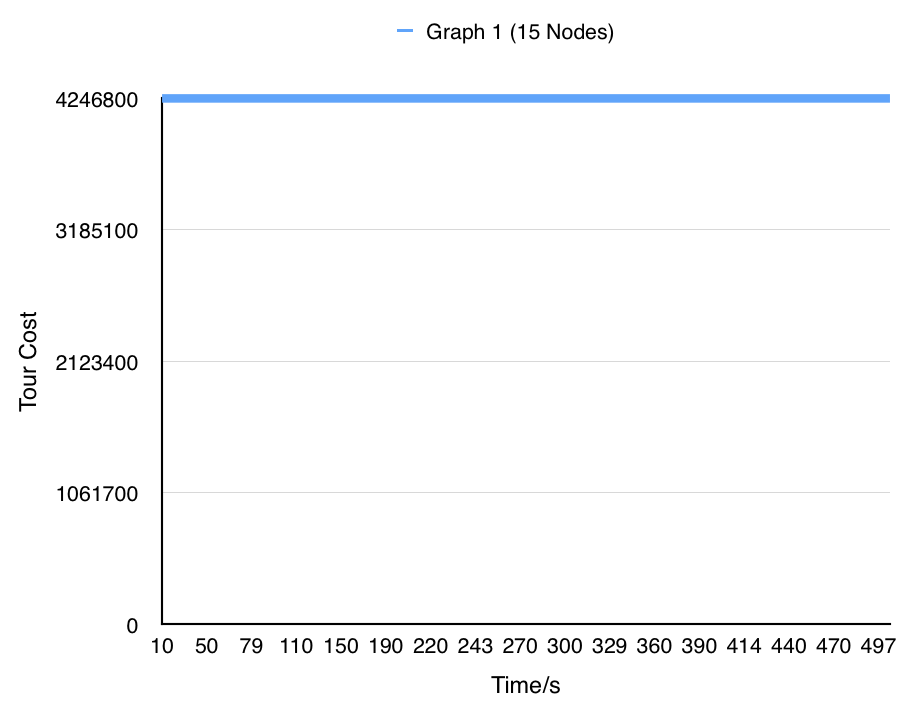
\includegraphics[scale=0.3]{fig1.png} \\
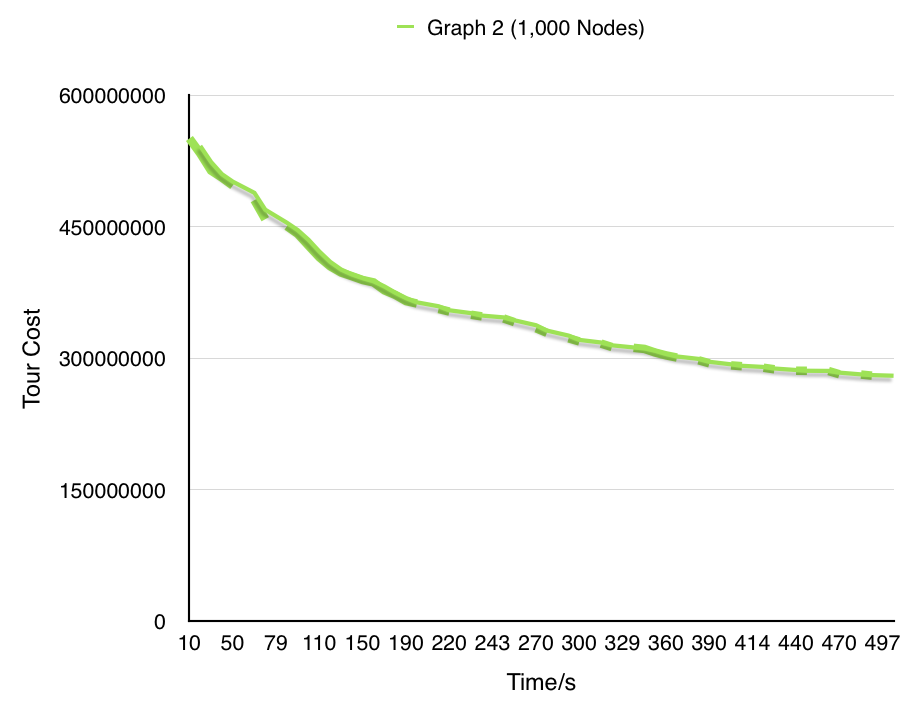
\includegraphics[scale=0.3]{fig2.png} \\
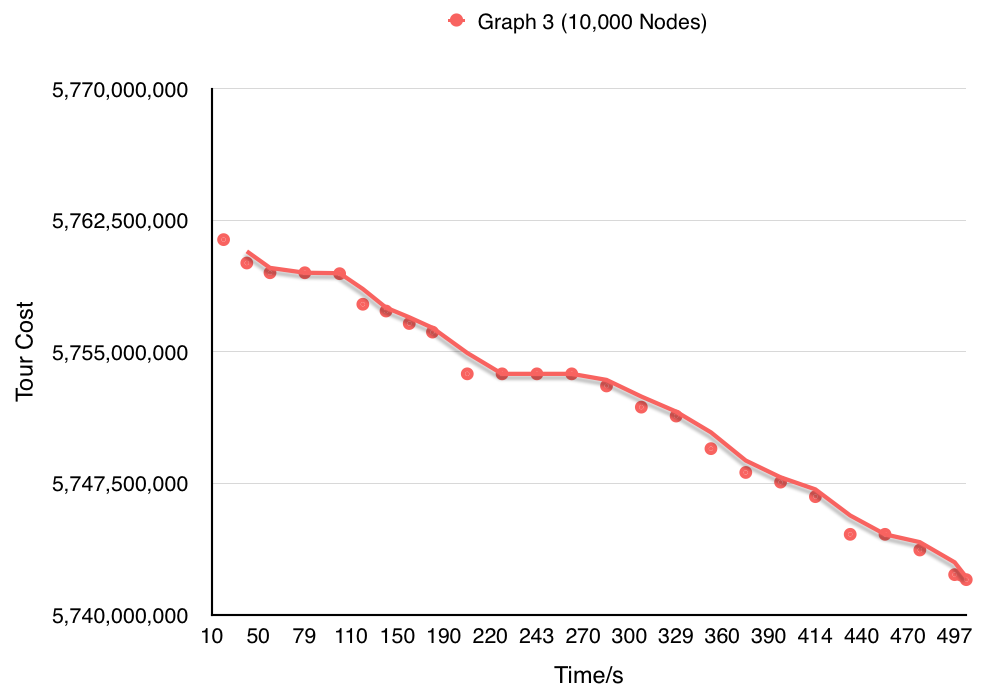
\includegraphics[scale=0.3]{fig3.png} 
\end{center}

There are several observations to be made from the graphs:
\begin{enumerate}
\item For a small-sized graph, the 2-opt algorithm with local search returns the optimal solution immediately. This solution is compared with the optimal solution produced by the Held-Karp algorithm.
\item For the medium-sized graph, as time increases, the cost of tour returned by the algorithm decreases at a decreasing rate. The cost returned by the algorithm starts to plateau at around 330s.
\item For the large-sized graph, the algorithm has to be ran much longer before it approaches the optimal solution.
\end{enumerate}

\section{Conclusions}

\section{Bibliography}
\bibliographystyle{plain}
\nocite{*}
\bibliography{biblio}
%%% End document
\end{document}